\usepackage{amsmath}
\allowdisplaybreaks[4]
\usepackage{amssymb}
\usepackage{graphicx}
\usepackage{fontawesome,pifont,oplotsymbl}
\usepackage{marvosym}
\usepackage{savesym}
\savesymbol{Cross}
\usepackage{bbding}
\restoresymbol{bb}{Cross}
\usepackage{tikz}
\usetikzlibrary{calc,angles,intersections,shapes.geometric,arrows,decorations.markings,arrows.meta,patterns.meta,patterns,fadings,
shadows,backgrounds}
\tikzfading[name=fade out, inner color=transparent!0,outer color=transparent!100]
\tikzfading[name=fade left, top color=transparent!0,bottom color=transparent!0,middle color=transparent!100]
\tikzfading[name=fade right,left color=transparent!0,right color=transparent!100]
\usepackage{graphicx}%chỉnh hình ảnh
\usepackage{pgfornament}
\usepackage{makecell}
\usepackage{array}
\newcolumntype{L}[1]{>{\raggedright\let
\newline\\\arraybackslash\hspace{0pt}}m{#1}}
\newcolumntype{C}[1]{>{\centering\let
\newline\\\arraybackslash\hspace{0pt}}m{#1}}
\newcolumntype{R}[1]{>{\raggedleft\let
\newline\\\arraybackslash\hspace{0pt}}m{#1}}
\renewcommand{\arraystretch}{1.25}
\usepackage[most,xparse,many]{tcolorbox}
\usepackage[explicit]{titlesec} %Gói thiết lập chương mục
\newcommand\circlenum[2][cyan]{\tikz[baseline=(char.base)]
{\node[shape=circle,inner sep=1pt,draw=#1,fill=#1!10,
font=\bfseries\footnotesize,minimum size=14pt,outer sep=0pt] (char) {#2};}}
\newcommand\circlenumH[2][cyan]{\tikz[baseline=(char.base)]
{\node[shape=circle,inner sep=0.5pt,draw=#1,%fill=#1!10,
font=\bfseries\footnotesize,minimum size=13pt,outer sep=0pt] (char) {#2};}}
\renewenvironment{center}
{\parskip=3pt\par\nopagebreak\centering}
{\par\noindent\ignorespacesafterend}
\usepackage{multicol}
\setlength{\multicolsep}{2pt plus 1pt minus 1pt}
%%%============================================%%%
\DeclareSymbolFont{symbolsC}{U}{txsyc}{m}{n}
\DeclareMathSymbol{\varparallel}{\mathrel}{symbolsC}{9}
\renewcommand{\parallel}{\mathbin{\!\raisebox{0.25pt}/\mkern-2mu\raisebox{0.25pt}/\!}}
\renewcommand{\backsim}{\ \mathord{\raisebox{0.025\baselineskip}{\rotatebox{90}{\fontfamily{qag}\selectfont S}}}\ }
\setlength\arraycolsep{2pt}
\newcommand{\hoac}[1]{\renewcommand{\arraystretch}{0.85}\left[\begin{aligned}#1\end{aligned}\right.}
\newcommand{\heva}[1]{\renewcommand{\arraystretch}{0.85}\left\{\begin{aligned}#1\end{aligned}\right.}
\DeclareSymbolFont{AMSb}{U}{msb}{m}{n}
\makeatletter
\DeclareSymbolFontAlphabet{\math@bb}{AMSb}
\AtBeginDocument{\protected\def\mathbb{\math@bb}}
\g@addto@macro\normalsize{
\setlength{\abovedisplayskip}{4pt}%
\setlength{\belowdisplayskip}{2pt}%
\setlength{\abovedisplayshortskip}{4pt}%
\setlength{\belowdisplayshortskip}{1pt}%
}
\makeatother
\def\bmod{\operatorname{mod}\,}
\makeatletter
\DeclareRobustCommand
\vdots{\,\vbox{\baselineskip3\p@ \lineskiplimit\z@
\hbox{.}\hbox{.}\hbox{.}}\,}
\makeatother
\usepackage[explicit]{titlesec} %Gói thiết lập chương mục
\titlespacing*{\subsection}{0pt}{3pt}{6pt}
\titleformat{\subsection}{}{}{0pt}{%
{{\large\bfseries\sffamily\Roman{subsection}. \MakeUppercase{#1}}}
}
\titlespacing*{\subsubsection}{0pt}{3pt}{6pt}
\newfont{\damsc}{uncbc8v at 15pt}
\newfont{\damss}{t5-lmssbx10 at 15pt}
\newfont{\damugq}{ugqb8v at 19pt}
\titleformat{\subsubsection}{}{}{0pt}{%
	{\bfseries\sffamily\color{darkmidnightblue}\arabic{subsubsection})\, #1}
}
\def\muctieu{}
\titleformat{\section}
{\filcenter\setcounter{bt}{0}\setcounter{ex}{0}}
{}
{0pt}
{%
 \begin{tikzpicture}
 \path (0,0) node[outer sep=11pt] (A){{\damsc Đề} {\damugq\arabic{section}}.\; {\damss\MakeUppercase{#1}}} ;
 \path[color=cyan!65] (A.south west) to [ornament=88] (A.south east); 
 \path[color=cyan!25] (A.north west) to [ornament=88] (A.north east);
 \end{tikzpicture}
}
 %%%=============================================%%%
\usepackage{fancyhdr}
\pagestyle{fancy}
\fancyhead[RE]{}
\fancyhead[LE]{\rightmark}
\fancyhead[LO]{}
\fancyhead[RO]{\rightmark}
\cfoot{}
\renewcommand{\headrulewidth}{0pt}
\renewcommand{\chaptermark}[1]{\markboth{\color{darkmidnightblue}\sffamily Chương \arabic{chapter}.\ {#1}}{}%
}
\renewcommand{\sectionmark}[1]{\markright{\color{darkmidnightblue}\slshape \thesection. #1}}
\usepackage{eso-pic}
\usepackage{qrcode}
\usepackage{miama}
\AddToShipoutPicture{
\ifodd\thepage
\begin{tikzpicture}[overlay,remember picture]
\path ($(current page.south east)+(135:1.5)$) node[path fading=fade out,fill=cyan!65,minimum size=15pt,double,inner sep=0.1pt,
regular polygon, regular polygon sides=4,shape border rotate=45,font=\normalsize\sffamily](char){\thepage\;}
node[minimum size=15pt,inner sep=0.1pt,
regular polygon, regular polygon sides=4,shape border rotate=45,font=\normalsize\sffamily](A){\thepage\;};
\path ($(current page.south west)+(45:1.5)+(0.75,-3pt)$) node[anchor=west] (B)%
{\color{darkmidnightblue}{\small\faAngleDoubleRight}{\Large\fmmfamily\, \footerinfo}};
\draw[thick,darkmidnightblue] ($(A.west)-(0.05,0)$)--($(B.east)+(0,3pt)$);
\end{tikzpicture}
\else
\begin{tikzpicture}[overlay,remember picture]
\path ($(current page.south west)+(45:1.5)$)
node[path fading=fade out,fill=cyan!65,minimum size=15pt,inner sep=0.1pt,
regular polygon, regular polygon sides=4,shape border rotate=45,font=\normalsize\sffamily] (char){\thepage\;}
node[minimum size=15pt,inner sep=0.1pt,
regular polygon, regular polygon sides=4,
shape border rotate=45,font=\normalsize\sffamily](A){\thepage\;};
\path ($(current page.south east)+(135:1.5)-(0.75,3pt)$) node[anchor=east] (B)%
{\color{darkmidnightblue}{\small\faAngleDoubleRight}{\Large\fmmfamily\, \footerinfo}};
\draw[thick,darkmidnightblue] ($(A.east)+(0.05,0)$)--($(B.west)+(0,3pt)$);
\end{tikzpicture}
\fi
}
\renewcommand{\thesection}{\S \arabic{section}.}
\tikzset{laphuong/.pic={
\path[pic actions,line join=round]
(0,0)--++(27.5:r)--++(152.5:r)--+(-152.5:r)--cycle
(0,0)--++(0,-r)--++(152.5:r)--+(0,r)--cycle
(0,0)--++(0,-r)--++(27.5:r)--+(0,r)--cycle;
}}
%%%================================================%%%
\newcounter{hd}[section]
\newtcolorbox{hd}{before skip=6pt,after skip=6pt,
left skip=-0.35cm,
boxsep=1pt,
enhanced,
top=0pt,
frame empty,
frame hidden,
opacityback=0,
code={\refstepcounter{hd}},
before upper={
\begin{tikzpicture}[declare function={r=0.165;},baseline=(char.base)]
\path (30:1.1*r) pic[fill=orange,draw=white]{laphuong};
\path (150:1.1*r) pic[fill=red!75!blue,draw=white]{laphuong};
\path (270:1.075*r) pic[fill=green!75!blue,draw=white]{laphuong};
\fill[darkmidnightblue] (60:{2.5*r})--+(4*r,0)--(7.5*r,0)--($(-60:{2.5*r})+(4*r,0)$)--+(-4*r,0) arc(-60:60:{2.5*r});
\draw[ultra thick,darkmidnightblue](0,0) circle (2.5*r) (8*r,0);
\path ($({4*r},0)+(0.5pt,-0.65pt)$) node[font=\bfseries\sffamily\color{gray!65}\large] (char){\thehd};
\path ({4*r},0) node[font=\bfseries\sffamily\color{white}\large] (char){\thehd};
\end{tikzpicture}}
}

\newtcolorbox{kttrongtam}{
enhanced,breakable,
before skip=6pt,after skip=6pt,
boxsep=9pt,
left=1cm,
right=0.25cm,
bottom=0pt,
frame empty,
frame hidden,
arc=7pt,
colback=orange!7,
sharp corners,
rounded corners=south,
colframe=orange!35,
boxrule=0pt,
borderline north={9pt}{0pt}{orange!65},
drop fuzzy shadow=gray!75,
overlay unbroken and first ={
\fill[orange,drop shadow={opacity=0.25,shadow xshift=1pt, shadow yshift=-1.5pt,shadow scale=1.05}] (frame.north west) coordinate (A)--+(2,0)--($(A)+(0,-1.25)$)--cycle;
\path ($(A)+(0.65,-0.15)$) coordinate (B) node{

\begin{tikzpicture}[x=3.65pt,y=3.65pt,xscale=-1]
\draw[thick,orange,fill=white] (-1,-4) to[out=50,in=-90,looseness=1.4] (-1,-3) to[out=-160,in=0]
(-2,-3.2) to[out=180,in=-120] (-2.7,-2) to[out=120,in=-120] (-2.9,-1.5)
to[out=120,in=-120] (-2.95,-1.1) to[out=60,in=-30] (-3.2,-0.9)
to[out=150,in=-120] (-3,0.4) to[out=60,in=-90] (-3,1.2)
to[out=90,in=90,looseness=1.8] (3.3,1.2)
to[out=-90,in=90,looseness=0.8] (2,-2)
to[out=-90,in=150,looseness=0.8] (3.2,-4) -- cycle;
\end{tikzpicture}
};
\tikzset{declare function={r=0.275;}}
\path (B) pic[fill=orange,draw=white]{laphuong};
}
}

\newenvironment{tomtat}{\begin{kttrongtam}}{\end{kttrongtam}}

\newcounter{lt}[section] %số điếm của môi trường luyện tập
\newtcolorbox{luyentap}{
enhanced,breakable,
before skip=6pt,after skip=6pt,
boxsep=9pt,
left=0.75cm,
right=0.15cm,
bottom=0pt,
frame empty,
frame hidden,
arc=5pt,
colback=green!7,
sharp corners,
rounded corners=south,
colframe=green!30!blue!45,
boxrule=0pt,
borderline north={9pt}{0pt}{green!50},
drop fuzzy shadow=gray!75,
overlay unbroken and first ={
\fill[green!80!black,drop shadow={opacity=0.25,shadow xshift=1pt, shadow yshift=-1.5pt,shadow scale=1.05}] (frame.north west) coordinate (A)--+(1.5,0)--($(A)+(0,-1.25)$)--cycle;
\path ($(A)+(0.5,-0.4)$) coordinate (B) node[font=\LARGE\color{gray!65}]{\faEdit};
\path ($(B)+(-1pt,1pt)$) node[font=\LARGE\color{yellow}]{\faEdit};
},
code={\refstepcounter{lt}},
before upper={
\circlenum{\thelt}
}
}

\newtcolorbox{bttuongtu}{
enhanced,breakable,
before skip=6pt,after skip=6pt,
boxsep=9pt,
left=0.75cm,
right=0.15cm,
bottom=0pt,
frame empty,
frame hidden,
arc=5pt,
colback=green!7,
sharp corners,
rounded corners=south,
colframe=green!30!blue!45,
boxrule=0pt,
borderline north={9pt}{0pt}{green!50},
drop fuzzy shadow=gray!75,
overlay unbroken and first ={
\fill[green!80!black,drop shadow={opacity=0.25,shadow xshift=1pt, shadow yshift=-1.5pt,shadow scale=1.05}] (frame.north west) coordinate (A)--+(1.5,0) coordinate (Bt)--($(A)+(0,-1.25)$)coordinate (Ct)--cycle;
\path ($(A)+(0.5,-0.4)$) coordinate (B) node[font=\LARGE\color{gray!65}]{\faEdit};
\path ($(B)+(-1pt,1pt)$) node[font=\LARGE\color{yellow}]{\faEdit};
\path (Bt)--(Ct) node[below=-2.5pt,sloped,pos=0.5,text=green!75!black]{\scriptsize\sffamily bài tập tương tự};
}
}
%%%=============Lưu ý===============%%%%
\newtcolorbox{luuy}{
enhanced,breakable,
before skip=6pt,after skip=6pt,
boxsep=9pt,
before skip=16pt,
left=0.75cm,
right=0.15cm,
bottom=0pt,
frame empty,
frame hidden,
arc=5pt,
colback=teal!7,
sharp corners,
rounded corners=south,
colframe=teal!55,
boxrule=0pt,
borderline north={9pt}{0pt}{teal!65},
drop fuzzy shadow=gray!75,
overlay unbroken and first ={
\fill[teal!80!black,drop shadow={opacity=0.25,shadow xshift=1pt, shadow yshift=-1.5pt,shadow scale=1.05}] (frame.north west) coordinate (A)--+(1.5,0)--($(A)+(0,-1.25)$)--cycle;
\draw[teal!80!black,ultra thick,rounded corners=2pt] ($(A)+(6pt,0)$)--++(0,9pt)--++(12pt,0)--+(0,-9pt)
($(A)+(9pt,0)$)--++(0,5pt)--++(6pt,0)--+(0,-5pt)
;
\draw[white,ultra thick,rounded corners=2pt] ($(A)+(18pt,0)$)--++(0,-15pt)--++(-8.5pt,0)--+(0,15pt);
}
}

\usetikzlibrary{shapes.symbols}

\usepackage{paracol}%chia cột có tùy chọn độ rộng
\columnratio{0.7}
\globalcounter{lt}
%%%=================Phan bt===================%%%
\newcounter{vd}
\definecolor{dnxanh}{HTML}{00CC99}
\definecolor{dndo}{HTML}{CC0033}
\NewTColorBox{boxvd}{+!O{}}{
enhanced,
fonttitle=\bfseries\sffamily\color{white},
title={\faGg\ Ví dụ~\thevd a},
colframe=white,
colback=white,
colbacktitle=white,
fonttitle=\bfseries,
coltitle=black,
attach boxed title to top left=
{yshift=-2mm-\tcboxedtitleheight,yshifttext=2mm-\tcboxedtitleheight/2},
boxed title style={
frame hidden,
outer arc=0pt,
arc=0pt,
top=1pt,
bottom=1pt,
left=0pt,
right=0pt
},
overlay unbroken and first={
\path
($ (title.north west) +(-2pt,0pt)$) coordinate (A)
($ (title.south west) +(-2pt,3pt)$) coordinate (B)
($ (title.south east)+(3pt,3pt) $) coordinate (C)
($ (title.north east)+(3pt,0) $) coordinate (D)
(intersection of C--B and frame.north east--frame.south east) coordinate (Et)
(intersection of A--D and frame.north east--frame.south east) coordinate (Ft)
($ (Et)-(4pt,0) $) coordinate (E)
($(Ft)-(4pt,0)$) coordinate (F);
\draw[line width=1.65pt,gray!25,rounded corners=3pt] ($ (frame.north west) +(0,-2pt)$) rectangle (frame.south east);
\path[fill=dnxanh!25,rounded corners=3pt]
(A)--(B)--(E)--(F)--cycle;
\path[fill=dnxanh!70!black,rounded corners=2pt]
(A)--(B)--([xshift=3pt]C)--([xshift=3pt]D)--cycle;
\path[left color=dndo,right color=dndo!80,rounded corners=3pt]
([xshift=-2pt]A)--([xshift=-2pt]B)--(C)--(D)--cycle;

\path ($ (A)!0.5!(B) +(9pt,0)$) node[anchor=west,font=\color{white}\bfseries\sffamily\selectfont]{{\faGg\ Ví dụ~\thevd}};

\path ($ (C)!0.5!(D) +(9pt,0)$) node[anchor=west,font=\color{dnxanh!70!black}\itshape]{#1};
},
top=\tcboxedtitleheight
}

\def\vdhead#1{\refstepcounter{vd}
\begin{boxvd}[#1]}
\def\vdend{
\end{boxvd}}
\newenvironment{vd}[1][]{\vdhead{#1}}{\vdend}

\usepackage{etoolbox}
\AtBeginEnvironment{vd}{
\renewcommand{\loigiai}[1]{
\end{boxvd}
\def\vdend{}
\par\noindent{\color{dndo}\reflectbox{\Large\WritingHand}\ {\fmmfamily\LARGE Lời giải.}}
#1
}
}
\usetikzlibrary{decorations.pathmorphing}
\NewEnviron{cauhoikd}{
\begin{center}

\begin{tikzpicture}
\node[cloud,cloud ignores aspect=true,cloud puffs=35,cloud puff arc=70,draw=cyan!65,fill=white,
text width=0.5\linewidth,font=\sffamily,drop shadow={opacity=0.25,color=cyan}]
(nA){\BODY};
\begin{scope}[rotate=5]
\draw[cyan,fill=white] ($(nA.south west)+(-2,0.5)$) coordinate (A) circle (0.6)
($(A)+(240:0.375)$) arc (240:310:0.35)
($(A)+(30:0.2)$) circle (2pt)
($(A)+(150:0.2)$) circle (2pt);
\draw[thin,cyan!65] (A) circle (0.675);
\draw[cyan!85,line cap=round,thick,shift={(A)}] (15:0.675) arc (15:165:0.675)
(-15:0.675) arc (-15:-165:0.675);
\fill[cyan] ($(A)+(150:0.185)$) circle (1pt)
($(A)+(30:0.185)$) circle (1pt);
\path ($(A)+(60:0.7)+(-45:1pt)$) node[rotate=5,font=\bfseries\LARGE\color{gray}]{?};
\path ($(A)+(60:0.7)$) node[rotate=5,font=\bfseries\LARGE\color{orange}]{?};
\end{scope}
\end{tikzpicture}
\end{center}}

\NewEnviron{trithuc}{
\begin{center}

\begin{tikzpicture}
\node[decorate,decoration={snake},segment length=15pt,draw=cyan!65,thick,
fill=white,text width=0.75\linewidth,font=\sffamily,drop shadow={opacity=0.25,color=cyan}]
(nA){\BODY};
\begin{scope}[rotate=5]
\draw[cyan,fill=white] ($(nA.north west)+(-1,-0.25)$) coordinate (A) circle (0.6)
($(A)+(240:0.375)$) arc (240:310:0.35)
($(A)+(30:0.2)$) circle (2pt)
($(A)+(150:0.2)$) circle (2pt);
\draw[thin,cyan!65] (A) circle (0.675);
\draw[cyan!85,line cap=round,thick,shift={(A)}] (15:0.675) arc (15:165:0.675)
(-15:0.675) arc (-15:-165:0.675);
\fill[cyan] ($(A)+(150:0.185)$) circle (1pt)
($(A)+(30:0.185)$) circle (1pt);
\path ($(A)+(60:0.7)+(-45:1pt)$) node[rotate=-5,font=\bfseries\LARGE\color{gray}]{\faLightbulbO};
\path ($(A)+(60:0.7)$) node[rotate=-5,font=\bfseries\LARGE\color{red}]{\faLightbulbO};
\end{scope}
\end{tikzpicture}
\end{center}}
\newcommand{\timhieuthem}{%
\par
\noindent
\hspace*{-0.65cm}
\begin{tikzpicture}[declare function={rt=0.65;d=sqrt(2)*rt;}]
\path (90:rt) coordinate (A)
(180:rt) coordinate (B)
(270:rt) coordinate (C)
(0:rt) coordinate (D)
([shift={(0.15,0)}]0:rt) coordinate (E)
($ (E)+(135:rt) $) coordinate (F)
($ (E)+(-135:rt) $) coordinate (G)
($ (A)!0.5!(F) $) coordinate (AF)
($ (D)!0.5!(E) $) coordinate (DE)
($ (C)!0.5!(G) $) coordinate (CG)
;
\path[transform canvas={shift={(-45:2.5pt)}},left color=darkmidnightblue!50,right color=darkmidnightblue!5]
(F)--(E)--(G)--+(1.25*\linewidth,0)--([turn]90:d)--cycle;
\path[outer color=darkmidnightblue!65!black,inner color=darkmidnightblue!80,rounded corners=2pt] (A)--(B)--(C)--(D)--cycle;
\draw[line width=0.65pt,darkmidnightblue,line cap=round,rounded corners=1.5pt]
(AF)--(DE)--(CG);
\draw[transform canvas={xscale=-1},line width=0.65pt,darkmidnightblue,line cap=round,rounded corners=1.5pt] (AF)--(DE)--(CG);
\path[left color=darkmidnightblue!90!black,right color=darkmidnightblue!50] (F)--(E)--(G)--+(1.25*\linewidth,0)--([turn]90:d)--cycle;
\path (-0.7pt,-0.3pt) node[inner sep=0pt,font=\Large\itshape\bfseries\color{gray},xscale=-1]{\faSearchPlus};
\path (-1pt,0) node[inner sep=0pt,font=\Large\itshape\bfseries\color{white},xscale=-1]{\faSearchPlus};
\path ([shift={(0.11,-0.01)}]E) node[align=left,anchor=west,font=\large\sffamily\bfseries\color{gray}]{TÌM HIỂU THÊM};
\path ([shift={(0.1,0)}]E) node[align=left,anchor=west,font=\large\sffamily\bfseries\color{white}]{TÌM HIỂU THÊM};
\end{tikzpicture}%
}

\newcommand{\baitap}{\par%
\noindent
\begin{tikzpicture}
\path[left color=black!25,right color=white] (0,0) --(5cm,0)--([turn]90:0.7cm)--([turn]90:5cm)--cycle;
\path[fill=darkmidnightblue] (0,0)--(0.7cm,0)--([turn]90:0.7cm)--([turn]90:0.7cm)--cycle;
\path[left color=darkmidnightblue,right color=white] (0,0)--(\linewidth,0)--([turn]90:1pt)--([turn]90:\linewidth)--cycle;
\path (0.75,-1.5pt) node[anchor=south west,font=\sffamily\bfseries\color{\mauchinh}]{BÀI TẬP};
\path (0.73,-2pt) node[anchor=south west,font=\sffamily\bfseries\color{cyan}]{BÀI TẬP};
\end{tikzpicture}
}


\newcounter{dang}
\newtcolorbox{dang}[1]{
fonttitle=\sffamily\bfseries,%fontupper=\itshape,
breakable,
enhanced jigsaw,
colbacktitle=\mauchinh,
coltitle=white,
colframe=\mauchinh,
colback=white,
sharp corners,
rounded corners=south,
borderline north={1pt}{0pt}{maudoilap},
drop fuzzy shadow=gray!75,
before skip=3mm,after skip=3mm,
left=2mm,right=2mm,top=2mm,bottom=2mm,
title style={left color=\mauchinh,right color=\mauchinh!65},
underlay unbroken and first={
\def\dai{0.75}
\pgfmathsetmacro{\daih}{\dai/cos(20)}
\def\cao{0.5}
\fill[\mauchinh!85!black,rounded corners=1pt,drop shadow={shadow xshift=1pt, shadow yshift=-1pt,fill=gray!65}]
([shift={(2*\dai,5pt)}]title.north west)
coordinate (A1)
--+(2*\dai,0) coordinate (A2)
--([turn]-90:\cao) coordinate (A3)
--([turn]-70:\daih)
--([turn]-40:\daih) coordinate (A4)
--cycle;
\begin{pgfonlayer}{background}
\fill[gray!65] (A1)--++(225:0.5)--+(1,0)--cycle;
\end{pgfonlayer}
\node[circle,draw=white,fill=maudoilap,line width=1pt, inner sep=3pt,text=white,font=\sffamily\bfseries] at ($(A1)!0.5!(A3)+(0,-5pt)$){\thedang};
\path([yshift=-1.5pt]A4) node[font=\sffamily\bfseries,text=white,anchor=east]{Dạng};
},
overlay middle and last={
\def\dai{0.75}
\pgfmathsetmacro{\daih}{\dai/cos(20)}
\def\cao{0.5}
\fill[left color=\mauchinh,right color=\mauchinh!65,draw=\mauchinh,line width=1.4pt] ($(frame.north west)+(0.7pt,13pt)$) rectangle ($(frame.north east)+(-0.7pt,-7pt)$);
\fill[\mauchinh!85!black,rounded corners=1pt,drop shadow={shadow xshift=1pt, shadow yshift=-1pt,fill=gray!65}]
([shift={(2*\dai,17pt)}]frame.north west)
coordinate (A1)
--+(2*\dai,0) coordinate (A2)
--([turn]-90:\cao) coordinate (A3)
--([turn]-70:\daih)
--([turn]-40:\daih) coordinate (A4)
--cycle;
\begin{pgfonlayer}{background}
\fill[gray!65] (A1)--++(225:0.5)--+(1,0)--cycle;
\end{pgfonlayer}
\node[circle,draw=white,fill=maudoilap,line width=1pt, inner sep=3pt,text=white,font=\sffamily\bfseries] at ($(A1)!0.5!(A3)+(0,-5pt)$){\thedang};
\path([yshift=0.5pt]A4) node[font=\sffamily\bfseries,text=white,anchor=east]{Dạng};
\path([yshift=0.5pt]A3) node[font=\sffamily\bfseries,text=white,anchor=west]{Phần tiếp theo};
},
title={\hspace*{2.9cm}\parbox{\textwidth-3cm}{#1}\refstepcounter{dang}},%
}
%%%========môi trường note==============%%%
\usepackage{relsize}
\newenvironment{note}{\begin{luuy}%
{\faBellO\ \relscale{0.9}{\usefont{T5}{put}{b}{sc} Lưu ý}}. \ignorespaces}{\end{luuy}}

\newenvironment{nx}{\begin{luuy}%
	{\faPaperclip\ \relscale{0.9}{\usefont{T5}{put}{b}{sc} Nhận xét}}. \ignorespaces}{\end{luuy}}

\newenvironment{pp}{\begin{luuy}%
	{\faSpinner\ \relscale{0.9}{\usefont{T5}{put}{b}{sc} Phương pháp}}. \ignorespaces}{\end{luuy}}

\newenvironment{phuongphap}{\begin{luuy}%
	{\faSpinner\ \relscale{0.9}{\usefont{T5}{put}{b}{sc} Phương pháp}}. \ignorespaces}{\end{luuy}}

\newcommand\khungct[1]
{\noindent
\begin{tikzpicture}[baseline=(char.base)]%
	\tikzstyle{khung} = [rectangle,draw=darkmidnightblue,inner sep=6pt,rounded corners]%
	\node [khung] (char){%
	$
	\; #1.\;
	$
	};%
\end{tikzpicture}}
\newenvironment{phantich}{\begin{luuy}%
	{\faGears\ \relscale{0.9}{\usefont{T5}{put}{b}{sc} Phân tích}}. \ignorespaces}{\end{luuy}}
\usepackage{amsxtra,amssymb,latexsym,amscd,amsfonts}
\renewcommand{\thesubsection}{\Roman{subsection}}
\renewcommand{\thesubsubsection}{\arabic{subsubsection}}
%%%============môi trường định lý============%%%
\newcounter{dl}
\newenvironment{dl}[1][]{\setcounter{dl}{\arabic{subsubsection}}\refstepcounter{subsubsection}\refstepcounter{dl}\ifblank{#1}{{\sffamily\bfseries\color{darkmidnightblue}\par\noindent\thedl) Định lý.\,}}%
{{\sffamily\bfseries\color{darkmidnightblue}\par\noindent\thedl) Định lý (#1).\,}}\itshape}{}
%%%============môi trường hq============%%%
\newcounter{hq}
\newenvironment{hq}[1][]{\setcounter{hq}{\arabic{subsubsection}}\refstepcounter{subsubsection}\refstepcounter{hq}\ifblank{#1}{{\sffamily\bfseries\color{darkmidnightblue}\par\noindent\thehq) Hệ quả.\,}}%
{{\sffamily\bfseries\color{darkmidnightblue}\par\noindent\thehq) Hệ quả (#1).\,}}\itshape}{}
%%%============môi trường tc============%%%
\newcounter{tc}
\newenvironment{tc}[1][]{\setcounter{tc}{\arabic{subsubsection}}\refstepcounter{subsubsection}\refstepcounter{tc}\ifblank{#1}{{\sffamily\bfseries\color{darkmidnightblue}\par\noindent\thetc) Tính chất.\,}}%
{{\sffamily\bfseries\color{darkmidnightblue}\par\noindent\thetc) Tính chất (#1).\,}}\itshape}{}
%%%============môi trường định nghĩa============%%%
\newcounter{dn}
\newenvironment{dn}[1][]{\setcounter{dn}{\arabic{subsubsection}}\refstepcounter{subsubsection}\refstepcounter{dn}\ifblank{#1}{{\sffamily\bfseries\color{darkmidnightblue}\par\noindent\thedn) Định nghĩa.\,}}%
{{\sffamily\bfseries\color{darkmidnightblue}\par\noindent\thedn) Định nghĩa (#1).\,}}}{}
\usepackage[loigiai]{ex_test}
\newcounter{bt}
\makeatletter
\renewcommand{\TrueEX}{\stepcounter{dapan}
 {\circEX{{\fontfamily{paq}\selectfont\Alph{dapan}}}} \ignorespaces}
\renewcommand{\FalseEX}{\stepcounter{dapan}
 {\circled{{\Alph{dapan}}}} \ignorespaces}
 
\def\tieudehinh{}
\newcommand{\hinhphai}[2]{%
\tcbsidebyside[
sidebyside adapt=right,
blanker,sidebyside gap=5mm,
sidebyside align=top seam,
]{%
{\color{dndo}\tieudehinh}%
#1
}{%
#2%
}
}
%%%================Lệnh immini================%%%
\renewcommand{\immini}[3][]{
\savebox{\imbox}{#3}
\tcbsidebyside[
sidebyside adapt=right,
blanker,sidebyside gap=5mm,
sidebyside align=top seam,
]{%
{\tieudehinh}#2
}{%
\usebox{\imbox}
}
}
\usepackage{miama}
\renewcommand{\theequation}{\arabic{equation}}
\usepackage{tkz-tab}
\usepackage{mathrsfs}
\usepackage{tkz-euclide}
\usepackage{tikz-3dplot,pgfplots}
\pgfplotsset{compat=1.15}
\usepgfplotslibrary{polar,fillbetween}
\usepackage{esvect}
\def\vec{\vv} %vector
\def\overrightarrow{\vv}
\makeatletter
\newcommand\xleftrightarrow[2][]{%
\ext@arrow 9999{\longleftrightarrowfill@}{#1}{#2}}
\newcommand\longleftrightarrowfill@{%
\arrowfill@\leftarrow\relbar\rightarrow}
\makeatother
\usepackage[american]{circuitikz}
\tikzset{>=stealth}

\definecolor{redex}{HTML}{A70E10}
\definecolor{tealex}{HTML}{0EA7A5}
\makeatletter
\RenewDocumentEnvironment{ex}{+!O{}O{}}{%
\ifblank{#1}{%
	\ifblank{#2}{%
		\@ifnextchar\immini{\gdef\tieudehinh{\bfseries\sffamily Câu \theex\ (1 \starlet).\,}}%
		{{\par\noindent\bfseries\sffamily Câu \theex\ (1 \starlet).\,}}%
	 }%blank#2true
	 {
		\@ifnextchar\immini{\gdef\tieudehinh{{\bfseries\sffamily Câu \theex } {(#2 \starlet).\,}}}%
		{{\par\noindent\bfseries\sffamily Câu \theex} {(#2 \starlet).\,}}%
	 }%blank#2false
	}{%
	\ifblank{#2}{%
		\@ifnextchar\immini{\gdef\tieudehinh{{\bfseries\sffamily Câu \theex} (\textit{#1}, 1 \starlet).\,}}%
		{{\par\noindent{\bfseries\sffamily Câu \theex} (\textit{#1}, 1 \starlet).
		}}%
	 }%blank#2true
	 {
		\@ifnextchar\immini{\gdef\tieudehinh{{\bfseries\sffamily Câu \theex } {(\textit{#1}, #2 \starlet).\,}}}%
		{{\par\noindent\bfseries\sffamily Câu \theex} {(\textit{#1}, #2 \starlet).\,}}%
	 }%blank#2false	
	}
}{\gdef\tieudehinh{}}
\makeatother
\AtBeginEnvironment{ex}{
	 \refstepcounter{ex}
	 \setcounter{numTrue}{0}%
	 \setcounter{numTrueSol}{0}%
 \def\dotEX{.}%
 \setcounter{numChoice}{0}%
	 \renewcommand{\loigiai}[1]{\gdef\tieudehinh{}\par\noindent%
	 {\reflectbox{\Large\WritingHand}\ {\fmmfamily\LARGE Lời giải.}} #1
	 \ifthenelse{\value{numTrueSol}>0}{
	 \hfill \textcolor{tealex}{\sffamily \faKey~\circlenum{\Alph{numTrueSol}}}
	 }{}
 }
} 
\Newassociation{EXsolh}{Solution}{ans}
\AtEndEnvironment{ex}{%
\ifnum\the\value{numTrue}=1
\scantokens{\begin{EXsolh}A\end{EXsolh}}%
\fi%
\ifnum\the\value{numTrue}=2
\scantokens{\begin{EXsolh}B\end{EXsolh}}%
\fi%
\ifnum\the\value{numTrue}=3
\scantokens{\begin{EXsolh}C\end{EXsolh}}%
\fi
\ifnum\the\value{numTrue}=4
\scantokens{\begin{EXsolh}D\end{EXsolh}}
\fi%
\ifnum\the\value{numTrue}=5
\scantokens{\begin{EXsolh}E\end{EXsolh}}%
\fi%
}

\makeatletter
\NewDocumentEnvironment{bt}{+!O{}O{}}{%
\ifblank{#1}{%
	\ifblank{#2}{%
		\@ifnextchar\immini{\gdef\tieudehinh{\bfseries\sffamily Bài \thebt\ (1 \starlet).\,}}%
		{{\par\noindent\bfseries\sffamily Bài \thebt\ (1 \starlet).\,}}%
	 }%blank#2true
	 {
		\@ifnextchar\immini{\gdef\tieudehinh{{\bfseries\sffamily Bài \thebt } {(#2 \starlet).\,}}}%
		{{\par\noindent\bfseries\sffamily Bài \thebt} {(#2 \starlet).\,}}%
	 }%blank#2false
	}{%
	\ifblank{#2}{%
		\@ifnextchar\immini{\gdef\tieudehinh{{\bfseries\sffamily Bài \thebt} (\textit{#1}, 1 \starlet).\,}}%
		{{\par\noindent{\bfseries\sffamily Bài \thebt} (\textit{#1}, 1 \starlet).\,}}%
	 }%blank#2true
	 {
		\@ifnextchar\immini{\gdef\tieudehinh{{\bfseries\sffamily Bài \thebt } {(\textit{#1}, #2 \starlet).\,}}}%
		{{\par\noindent\bfseries\sffamily Bài \thebt} {(\textit{#1}, #2 \starlet).\,}}%
	 }%blank#2false	
	}
}{\gdef\tieudehinh{}}
\makeatother

\AtBeginEnvironment{bt}{
	 \refstepcounter{bt}
	 \renewcommand{\loigiai}[1]{\gdef\tieudehinh{}\par\noindent%
	 {\reflectbox{\Large\WritingHand}\ {\fmmfamily\LARGE Lời giải.}} #1
	 }
} 

\raggedbottom
\usepackage{intcalc}
\newcounter{itemcounth}
\newcommand{\bangdapan}[1]{%
\setcounter{itemcounth}{0}
\begin{center}
	{\large \bfseries\sffamily BẢNG ĐÁP ÁN}
	\medskip 
	
	\begin{minipage}{16cm}
		\setcounter{itemcounth}{0}
		\RenewEnviron{Solution}[1]{%
		\addtocounter{itemcounth}{1}
		\ifodd\intcalcDiv{\value{itemcounth}-1}{10}
		\tikz{\path (0,0) node[draw=maudoilap,thick,inner sep=3pt,text width=1.2cm,minimum height=0.65cm,
		rounded corners=3pt,outer sep=0pt,fill=yellow!5]{%
		{\textbf{##1}}\hfill
		{\textbf{\BODY}}%
		};
		}\ignorespaces
		\else
		\tikz{\path (0,0) node[draw=\mauchinh,thick,inner sep=3pt,text width=1.2cm,minimum height=0.65cm,
		rounded corners=3pt,outer sep=0pt,fill=yellow!5]{%
		{\textbf{##1}}\hfill
		{\textbf{\BODY}}%
		};
		}\ignorespaces
		\fi
		\ifthenelse{\equal{\intcalcMod{\value{itemcounth}}{10}}{0}}
		{\par\noindent\ignorespaces}{\hspace*{-6pt}}
		}
		\noindent
		\input{Ans/#1}
	\end{minipage}
\end{center}%
}
\newcommand{\Pointilles}[2][1.1]{%
 \par\nobreak
 \noindent\rule{0pt}{1.1\baselineskip}%
 \foreach \i in {1,...,#2}{%
 \ifnum\i=1
 \noindent\makebox[\linewidth]{\rule{0pt}{#1\baselineskip}\reflectbox{\Large\WritingHand}\dotfill}\endgraf
 \else
 \noindent\makebox[\linewidth]{\rule{0pt}{#1\baselineskip}\dotfill}\endgraf
 \fi
 }
}

\newcommand{\DoiThanhOly}[1]{
\setbox0=\vbox{\hbox{
\noindent\begin{minipage}{\linewidth}%
#1 aaaaa
\end{minipage}
}}
\linepar=\ht0
\pgfmathparse{int((\linepar-\fboxsep)/(\lineheight)+1)}
\let\mydong\pgfmathresult	\ifnum\pgfmathresult>3
		\begin{center}
			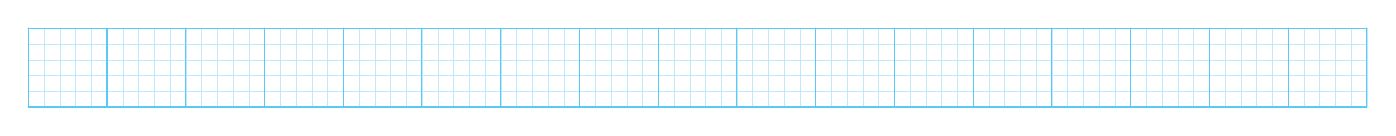
\begin{tikzpicture}
				\draw[cyan!25,ultra thin,step=0.2] (0,0) grid +(17,\mydong);
				\draw[cyan!65] (0,0) grid +(17,\mydong);
			\end{tikzpicture}
		\end{center}
	\else
	\noindent%
		\begin{center}
			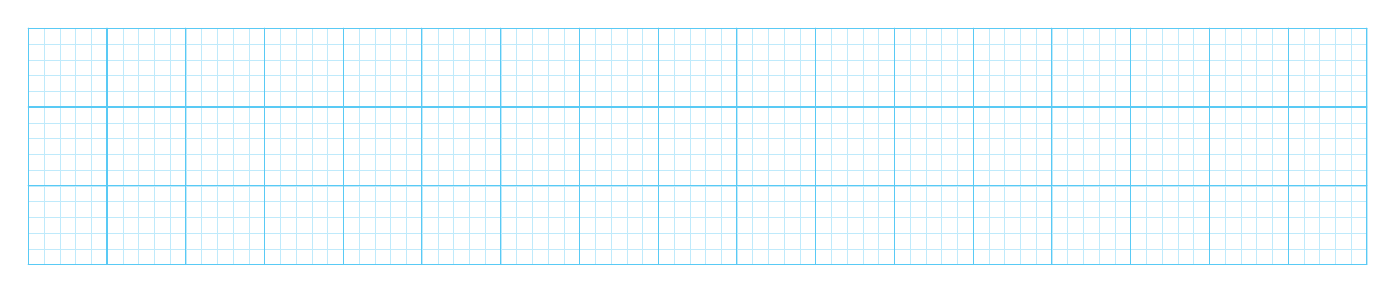
\begin{tikzpicture}
				\draw[cyan!25,ultra thin,step=0.2] (0,0) grid +(17,3);
				\draw[cyan!65] (0,0) grid +(17,3);
			\end{tikzpicture}
		\end{center}
	\fi
}

\newcommand{\DoiThanhDongKe}[1]{
\setbox0=\vbox{\hbox{
\noindent\begin{minipage}{\linewidth}%
#1 aaaaa
\end{minipage}
}}
\linepar=\ht0
\pgfmathparse{int((\linepar-\fboxsep)/(\lineheight)+1)}
	\ifnum\pgfmathresult>3
	\noindent%
		\Pointilles{\pgfmathresult}
	\else
	\noindent%
		\Pointilles{3}
	\fi
}

\newcommand{\DoiThanhDongKeH}[1]{
\setbox0=\vbox{\hbox{
\noindent\begin{minipage}{\linewidth}%
#1 aaaaa
\end{minipage}
}}
\linepar=\ht0
\pgfmathparse{int((\linepar-\fboxsep)/(0.85\lineheight)+1)}
	\ifnum\pgfmathresult>3
	\noindent%
		\Pointilles{\pgfmathresult}
	\else
	\noindent%
		\Pointilles{4}
	\fi
}
%%%=============================================%%%
\def\dongkeex{
	\AtBeginEnvironment{ex}{
		\renewcommand{\loigiai}[1]{%
	 \DoiThanhDongKe{##1}
		}
	}
}

%%%=============================================%%%
\def\Olyex{
	\AtBeginEnvironment{ex}{
		\renewcommand{\loigiai}[1]{%
	 \DoiThanhOly{##1}
		}
	}
}

%%%=============================================%%%
\def\dongkeHaicotex{
	\AtBeginEnvironment{ex}{
		\renewcommand{\loigiai}[1]{
			\begin{multicols}{2}			
				\DoiThanhDongKeH{##1}
			\end{multicols}
		}
	}
}

%%%=============================================%%%
\def\tatloigiaiex{%
	\AtBeginEnvironment{ex}{\renewcommand{\loigiai}[1]{}}
}

%%%=============================================%%%
\def\hienthiloigiaiex{%
	\AtBeginEnvironment{ex}{
	\renewcommand{\loigiai}[1]{%
	\par\noindent%
	{\color{dndo}\reflectbox{\Large\WritingHand}\ {\fmmfamily\LARGE Hướng dẫn}} \faKey\ \circlenum{\Alph{numTrue}} ##1
	}
	}
}

%%%=============================================%%%
\def\dongkebt{
	\AtBeginEnvironment{bt}{
		\renewcommand{\loigiai}[1]{
	 \DoiThanhDongKe{##1}
		}
	}
}

%%%=============================================%%%
\def\Olybt{
	\AtBeginEnvironment{bt}{
		\renewcommand{\loigiai}[1]{
	 \DoiThanhOly{##1}
		}
	}
}
%%%=============================================%%%
\def\dongkeHaicotbt{
	\AtBeginEnvironment{bt}{
		\renewcommand{\loigiai}[1]{
			\begin{multicols}{2}			
				\DoiThanhDongKeH{##1}
			\end{multicols}
		}
	}
}

%%%=============================================%%%
\def\tatloigiaibt{%
	\AtBeginEnvironment{bt}{\renewcommand{\loigiai}[1]{}}
}

%%%=============================================%%%
\def\hienthiloigiaibt{%
	\AtBeginEnvironment{bt}{
	\renewcommand{\loigiai}[1]{%
	\par\noindent%
	{\color{dndo}\reflectbox{\Large\WritingHand}\ {\fmmfamily\LARGE Hướng dẫn}} ##1
	}
	}
}

%%%=========================================%%%
\Newassociation{giaibt}{loigiaibt}{ansbt}
\def\luuloigiaibt{
	\AtBeginEnvironment{bt}{
		\renewcommand{\loigiai}[1]{%
		 \scantokens{%
		 \begin{giaibt}
		 ##1
		 \end{giaibt}}
		}
	}
}

\NewTColorBox{ansbt}{m}{
	 breakable,
	 enhanced,
	 outer arc=0pt,
	 arc=0pt,
	 colframe=white,
	 frame hidden,
	 left=-6pt,right=0pt,top=0pt,
	 colback=white,
	 attach boxed title to top left,
	 boxed title style={
	 colback=white,
	 outer arc=0pt,
	 arc=0pt,
	 top=1pt,
	 bottom=1pt,
	 left=3pt,
	 right=3pt,
	 colframe=white
 },
 fonttitle=\bfseries\sffamily\selectfont\color{white},
 title={HDBT~#1},
 overlay unbroken and first={
 \path (title.north west) coordinate (A)
 ($ (title.south west) +(-4pt,0pt)$) coordinate (B)
 (title.south east) coordinate (C)
 ($ (title.north east)+(4pt,0) $) coordinate (D);
 \path[rounded corners=2pt,fill=\mauchinh,
 preaction={transform canvas={shift={(-45:2pt)}},left color=\mauchinh!45,right color=\mauchinh!25}] 
 (A)--(B)--(C)--(D)--cycle;
 \path (A)--(C) node[midway,font=\color{white}\bfseries\sffamily\selectfont](Bai){\textsl{HDBT~#1}};
 \draw[rounded corners=2pt,thick,\mauchinh] ([xshift=-3pt]B) coordinate (Bt)
 --([shift={(-2pt,2pt)}]A)--+(\linewidth,0) coordinate (Ct);
 \fill[\mauchinh] (Bt) circle (1pt) (Ct) circle (2pt);
}
}
\renewenvironment{loigiaibt}[1]{\begin{ansbt}{#1}}{\end{ansbt}} %%%=====================Muc luc============================%%%
 \usepackage{titletoc}
 \usepackage[colorlinks]{hyperref}
 \patchcmd{\tableofcontents}{\contentsname}{\sffamily\contentsname}{}{}
 \makeatletter
 \renewcommand{\numberline}[1]{#1.~}
 \titlecontents{section}[1.5cm]{{\textcolor{dnxanh}\faApple}\ 
 \hypersetup{linkcolor=black}\vspace*{0.15\baselineskip}\sffamily\bfseries{\thecontentslabel.\;}}{}{}
 {\titlerule*[0.65pc]{.}\thecontentspage}
 \makeatletter
 \renewcommand{\tableofcontents}{%
 \newpage
 \markboth{Mục lục}{Mục lục}
 %\renewcommand{\rightmark}{Mục lục}
 \begin{center}
 \begin{tcolorbox}[enhanced,hbox,
 left=8mm,right=8mm,boxrule=0.55pt,
 bottom=3pt,
 colback=white,colframe=black,
 %drop fuzzy midday shadow=black!50!yellow,
 drop lifted shadow=black!50!yellow,arc is angular,
 before=\par\vspace*{-1mm},after=\par\bigskip]
 {\Large\bfseries\sffamily MỤC LỤC} 
 \end{tcolorbox}
 \end{center}
 \vskip-0.35cm
 \@starttoc{toc}}
 \makeatother
\def\phangiac(#1,#2,#3)(#4){
	\path ($ (#2)!1cm!(#1)$)  coordinate (Am)
		($ (#2)!1cm!(#3)$)  coordinate (Bm)
		($(Bm)+(Am)-(#2) $) coordinate (Cm)
		(intersection of #1--#3 and #2--Cm) coordinate (#4);}
\newcommand{\gocv}[4][black]{\draw[#1] ($(#3)!5pt!(#2)$)--($(#3)!2!($($(#3)!5pt!(#2)$)!.5!($(#3)!5pt!(#4)$)$)$)--($(#3)!5pt!(#4)$);}
\newcommand{\gv}[4][black]{\draw[#1] ($(#3)!5pt!(#2)$)--($(#3)!2!($($(#3)!5pt!(#2)$)!.5!($(#3)!5pt!(#4)$)$)$)--($(#3)!5pt!(#4)$);}
\def\gocvg(#1,#2,#3){\draw[black]($(#2)!6pt!(#1)$)--($($(#2)!6pt!(#1)$)+($(#2)!6pt!(#3)$)-(#2)$)--($(#2)!6pt!(#3)$);}
\def\khvuong(#1,#2,#3){
		\path ($(#2)!3mm!(#1)$) coordinate (#2#1)
		($(#2)!3mm!(#3)$) coordinate (#2#3);
		\draw[black] (#2#1)--($(#2#1)+(#2#3)-(#2)$)--(#2#3);}
\def\khgoc(#1,#2,#3){
\begin{scope}
	\clip (#1)--(#2)--(#3);
	\draw[black] (#2) circle (3mm);
\end{scope}}
\tkzSetUpPoint[shape =circle,color=black,size=1pt,fill=white]
\tikzset{every picture/.append style={line join=round,line cap=round} }